\documentclass[11pt, a4paper]{article}
\usepackage{graphicx}
\usepackage{amsmath}
\usepackage{listings}
\usepackage{minted}

\title{Assignment No 9: The Digital Fourier Transform} 

\author{Sakthi Harish D T (EE19B054)} 

\date{April $29^{th}$, 2021} 
\begin{document}		

\maketitle 
\section*{Abstract}
In this assignment we will,
\begin{enumerate}
    \item Try computing the Digital Fourier transforms of different signals under various sets of sampling points.
    \item Visualize the Fourier transforms and compare them with the actual values computed by hand.
    \item Compute the DFT of the given Gaussian input signal and calculate the error in the DFT computed. 
    
For the computations of the Discrete fourier transform (DFT), we use the \texttt{numpy.fft()} package.
\end{enumerate}

\section{Working through the given examples:}
In this section, we try computing the DFT of the given examples in the question,
\subsection{Error of DFT using Random function x:}
Firstly we try evaluating the DFT of a random function, using this, we again reconstruct the time domain signal, then compute the absolute error between the two.

Magnitude of maximum error between actual and Regenerated values of the random sequence: 2.237726045655905e-16. We see that the maximum error is in the order of $10^{-15}$, and hence the method of computation of DFT using \texttt{numpy.fft()} is pretty accurate.

The Actual value of x and the computed value of x is shown below in the graph. We can see that both the values coincide .
\begin{figure}[H]
\centering
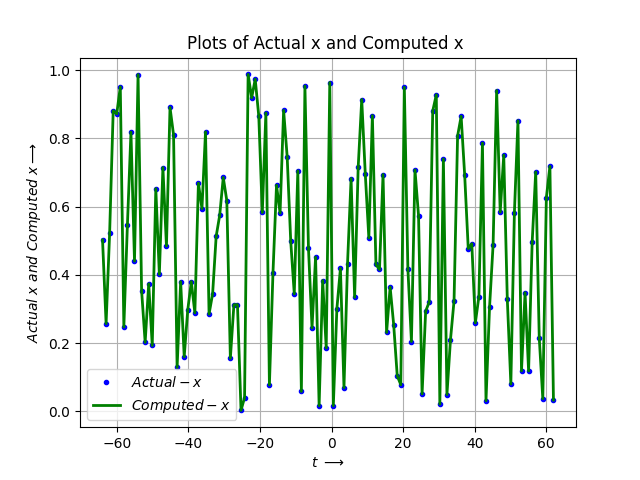
\includegraphics[scale=0.6]{Figure_0.png}
\label{fig:fig_0}
\caption{Actual and Estimated value of random function}
\end{figure}

We can see that the computation of DFT is very accurate using \texttt{numpy.fft()}.

\subsection{Spectrum of $sin(5t)$:}
In this part, we compute the spectrum for $sin(5t)$ and  we plot the phase and magnitude of the DFT,

\begin{figure}[H]
\centering
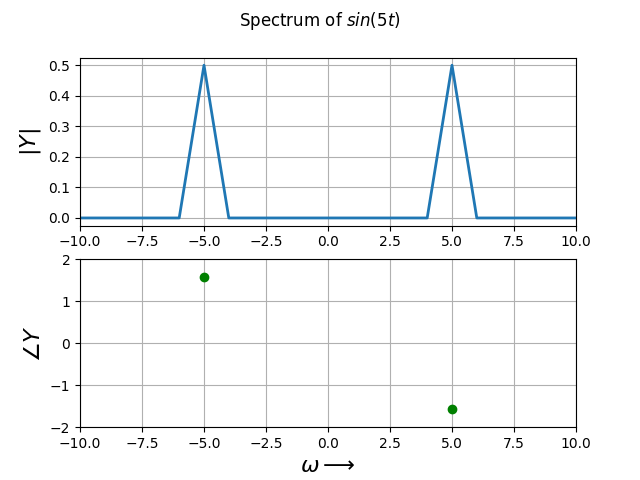
\includegraphics[scale=0.6]{Figure_1.png}
\label{fig:fig_1}
\caption{Spectrum of $sin(5t)$}
\end{figure}

This is as expected, because:
\begin{equation}
sin(5t) = \frac{1}{2j}(e^{5jt}-e^{-5jt})
\end{equation}
So, the frequencies present in the DFT of $sin(5t)$ are $\omega = \pm5\ rad/sec$, and the phase associated with them is $\phi = \mp \frac{\pi}{2}\ rad/sec$ respectively. This is exactly what is shown in the above plot.

\subsection{Spectrum of $(1+0.1cos(t))cos(10t)$:}
We have the equation,
\begin{equation}
    (1+0.1cos(t))cos(10t) = \frac{1}{2}(e^{10jt}+e^{-10jt}) + 0.1\cdot\frac{1}{2}\cdot\frac{1}{2}(e^{9jt} + e^{-9jt} + e^{11jt} + e^{-11jt})
\label{eqModAmp}
\end{equation}
    
Writing $(1+0.1cos(t))cos(10t)$ in a different form as shown in \eqref{eqModAmp}, we observe that the frequencies present in the signal are $\omega = \pm 10\ rad/sec$, $\omega = \pm 9\ rad/sec$ and $\omega = \pm 11\ rad/sec$. Thus we expect the spectrum also to have non-zero magnitudes only at these frequencies.\\


Now plotting the spectrum of the signal we get,
\begin{figure}[H]
\centering
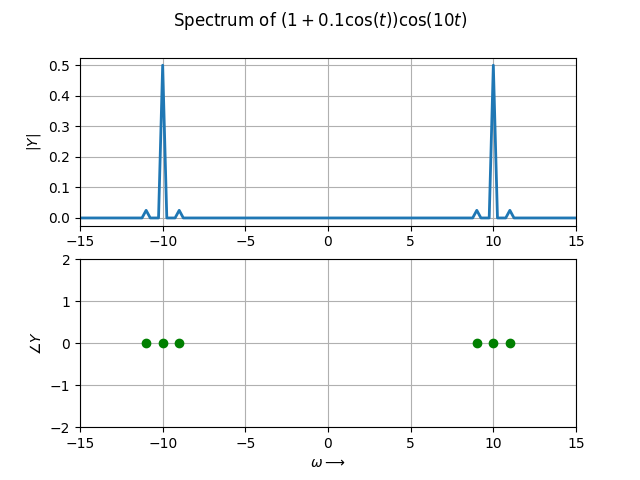
\includegraphics[scale=0.6]{Figure_2.png}
\caption{Spectrum of $(1+0.1cos(t))cos(10t)$}
\label{fig:fig_3}
\end{figure}

As expected, we see that the peaks occur only at the frequencies of $\omega = \pm 9\ , \pm 10\ , \pm 11\ rad/sec$.
\clearpage

\section{Spectra of $sin^3(t)$ and $cos^3(t)$:}
\subsection{Spectrum of $sin^3(t)$:}
We know that,

\begin{gather}
    sin^3(t) = \frac{3}{4}sin(t) - \frac{1}{4}sin(3t)
\end{gather}

So, we expect peaks $\omega = \pm 1\ rad/sec$ and $\omega = \pm 3\ rad/sec$.

The Spectrum of $sin^3(t)$ is,
\begin{figure}[H]
    \centering
    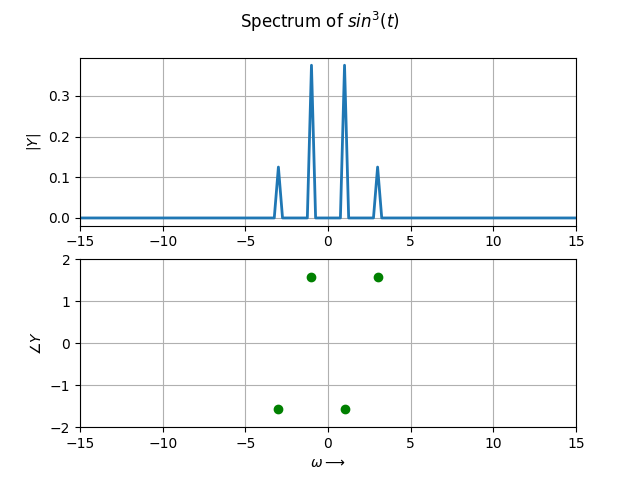
\includegraphics[scale=0.65]{Figure_3.png}
    \caption{Spectrum of $sin^3(t)$}
    \label{fig:sin^3t}
\end{figure}
\subsection{Spectrum of $cos^3(t)$:}
We know that,
\begin{gather}
    cos^3(t) = \frac{3}{4}cos(t) + \frac{1}{4}cos(3t)
\end{gather}
Here also, we expect peaks $\omega = \pm 1\ rad/sec$ and $\omega = \pm 3\ rad/sec$. \newline
The Spectrum of $cos^3(t)$.
\begin{figure}[H]
    \centering
    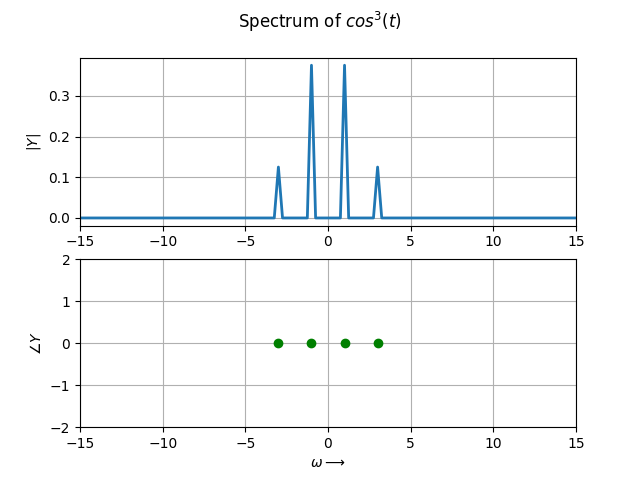
\includegraphics[scale=0.65]{Figure_4.png}
    \caption{Spectrum of $cos^3(t)$}
    \label{fig:cos^3t}
\end{figure}

We see that the peaks occur at the expected frequencies. The phase of $cos^3(t)$ is 0 as expected for a Cosine function.

\section{Spectrum of $cos(20t + 5cos(t))$}

\begin{figure}[H]
\centering
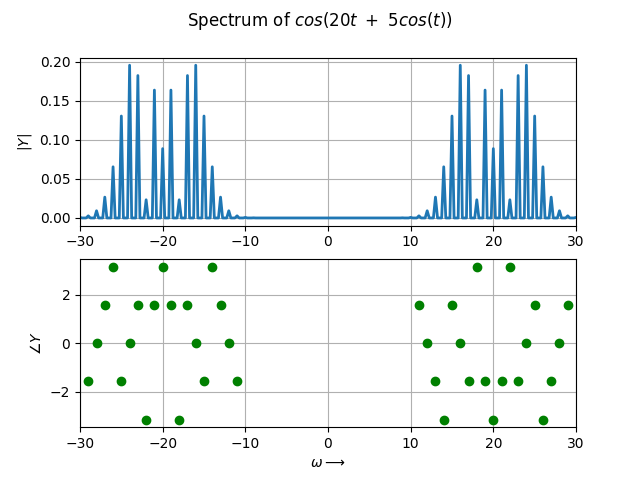
\includegraphics[scale=0.62]{Figure_5.png}
\caption{Spectrum of $cos(20t + 5cos(t))$}
\label{fig:freqMod}
\end{figure}
The spectrum of $cos(20t + 5cos(t))$ can be seen above, \newline
We see that the plot is phase modulated i.e there is peaking at the points of $\omega=20$ and $\omega=-20$, also in this case we have plotted the phase spectrum only for the frequencies where the magnitude spectrum is greater $10^-3$, and thus we see the phase points to be scattered around the points $\omega=20$ and $\omega=-20$.

\section{Spectrum of the Gaussian}
In this section we try finding the spectrum of the Gaussian signal $x(t)=exp(-t^2/2)$, we compute the spectrum using the $numpy.fft()$ package and as well compare with the actual spectrum computed by hand. The point of having a special attention on the spectrum of a Gaussian is that the signal is not band limited. 

By actual calculation of the spectrum of a Gaussian signal we get it's spectrum as well to be a Gaussian in $\omega$,
\begin{gather}
    x(t) = exp(-t^2/2)\\
    X(\omega) = exp(-{\omega}^2/2)/\sqrt{2\pi}
\end{gather}

Now looking at the plots of the computed spectrum and the actual spectrum,
\begin{figure}[H]
\centering
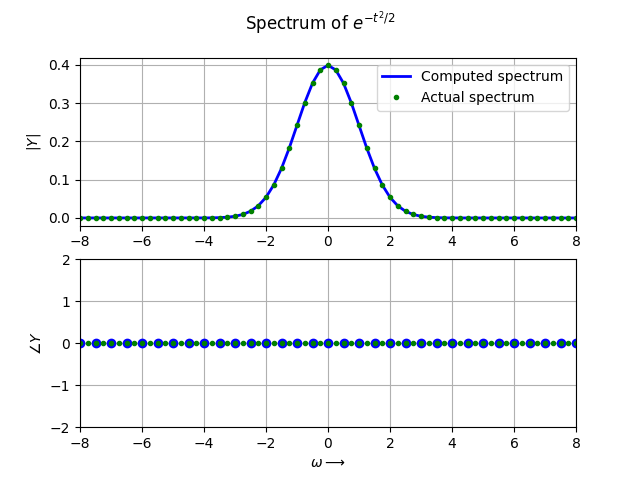
\includegraphics[scale=0.7]{Figure_6.png}
\caption{Comparison of the actual and estimated spectrum of the Gaussian}
\label{fig:gauss}
\end{figure}

As we can see from the above figure that both the estimated and the actual spectrum is almost same.

The Magnitude of mean error between actual and computed values of the Gaussian: 0.007812500000000014

\section*{Conclusion}
To conclude, we have seen the following in this assignment,
\begin{enumerate}
    \item We have worked through the examples taught in class.
    \item We have tried computing the various Discrete time Fourier transforms of various signals like \texttt{random function, sin(5t), Gaussian, etc.,}
    \item We have used the method of Fast Fourier transform in order to compute the Discrete time Fourier transform.
    \item The method of FFT worked well for the signals with samples in $2^k$ as the method divides the signal into the groups of 2 and computes the transform.
    \item The \texttt{numpy.fft()} package is very accurate to calculate the DFT of functions.
\end{enumerate}

\end{document}
